\documentclass[a4paper,fontset=fandol]{ctexart}

\usepackage{amsmath,amssymb,amsthm,physics,fancyhdr,geometry,hyperref,graphicx,enumitem,upgreek,booktabs}

\geometry{vmargin=2cm,hmargin=2.5cm}

\pagestyle{fancy}
\fancyhf{}
\fancyfoot[C]{\thepage}
\renewcommand{\headrulewidth}{0pt}

\usepackage{titlesec}
\titleformat{\section}
{\normalfont\Large\bfseries}{观测\thesection:}{0.5em}{}

\newcommand{\points}[1]{\par % 确保换行
	\noindent % 取消缩进
	\hfill (#1分)% 右对齐并添加分数
	\vspace{1em}
	}

%\parskip=0.5em

\hypersetup{colorlinks}

\begin{document}
	{
		\Large\bfseries\noindent 观测:\hspace{0.5em}流程
	}
	
	你有30分钟的时间来阅读问题并规划你的观测. 不要与其他参与者交谈. 当监考员出示``现在开始''的信号时, 请按照指示前往望远镜位置, 并随身携带试题、写字板和笔/铅笔 (望远镜处将提供红色光源) . 与其他参与者保持距离, 不要与他们交谈. 向你的助手出示你的徽章和代码. 
	
	当所有参与者准备好后, 你将有总共30分钟的时间来完成观测任务. 30分钟结束时, 带着你的纸张和写字板 (留下光源), 等待离开观测位置. 
	
	按照指示返回准备大厅. 与其他参与者保持距离, 不要与他们交谈. 
	
	你将另有30分钟来处理您的观测结果并完成答题 (将提供计算器、几何工具等) . 如果你遇到任何技术问题, 可以在答题纸上的表格中为你的团队负责人写一份报告. 30分钟结束时, 将你的答题纸和报告放入信封, 并在你的桌子上等待, 直到被指示离开大厅. 
	
	\vspace{5em}
	{
		\Large\bfseries\noindent 观测:\hspace{0.5em}指导说明
	}
	
	科学家们发现了一艘坠毁的外星飞碟. 在货舱深处的高处, 他们找到了几个屏幕, 这些屏幕正在传输天空的视图, 并且已经设置了望远镜, 以便让你从甲板的位置清楚地看到它们. 使用你的望远镜观察屏幕上的 (模拟) 目标, 并记录你的结果. 
	
	对面有5个屏幕: 中央的那个将显示问题1和2的视频, 其他四个将显示问题3和4的静态图像. 两个靠近中心的屏幕将显示问题3的 (相同) 图像, 而两个外侧的屏幕将显示问题4的 (相同) 图像. 将你的望远镜指向离你最远的屏幕. 
	
	\begin{figure}[!h]
		\centering
		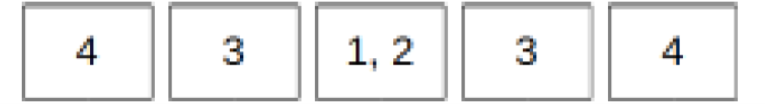
\includegraphics{fig/1.png}
	\end{figure}
	
	你将有总共30分钟的时间来完成观测比赛, 但问题1和2只展示一次: 就像真实的观测一样, 你只有一次机会收集数据. 将有两个时钟显示剩余时间. 
	
	在比赛开始时, 中央屏幕上的一个时钟将显示观测者所在地的模拟时间. 通过望远镜看时, 时钟将具有正确的方向. 时间将显示3分钟后消失; 利用这个来设定你的观测开始时间. 
	
	注意: 视频和静态图像的视场比例尺是不同的. 
	
	\newpage
	{
		\Large\bfseries\noindent 观测:\hspace{0.5em}星图1 (问题1与问题2)
	}
	
	\begin{figure}[!h]
		\centering
		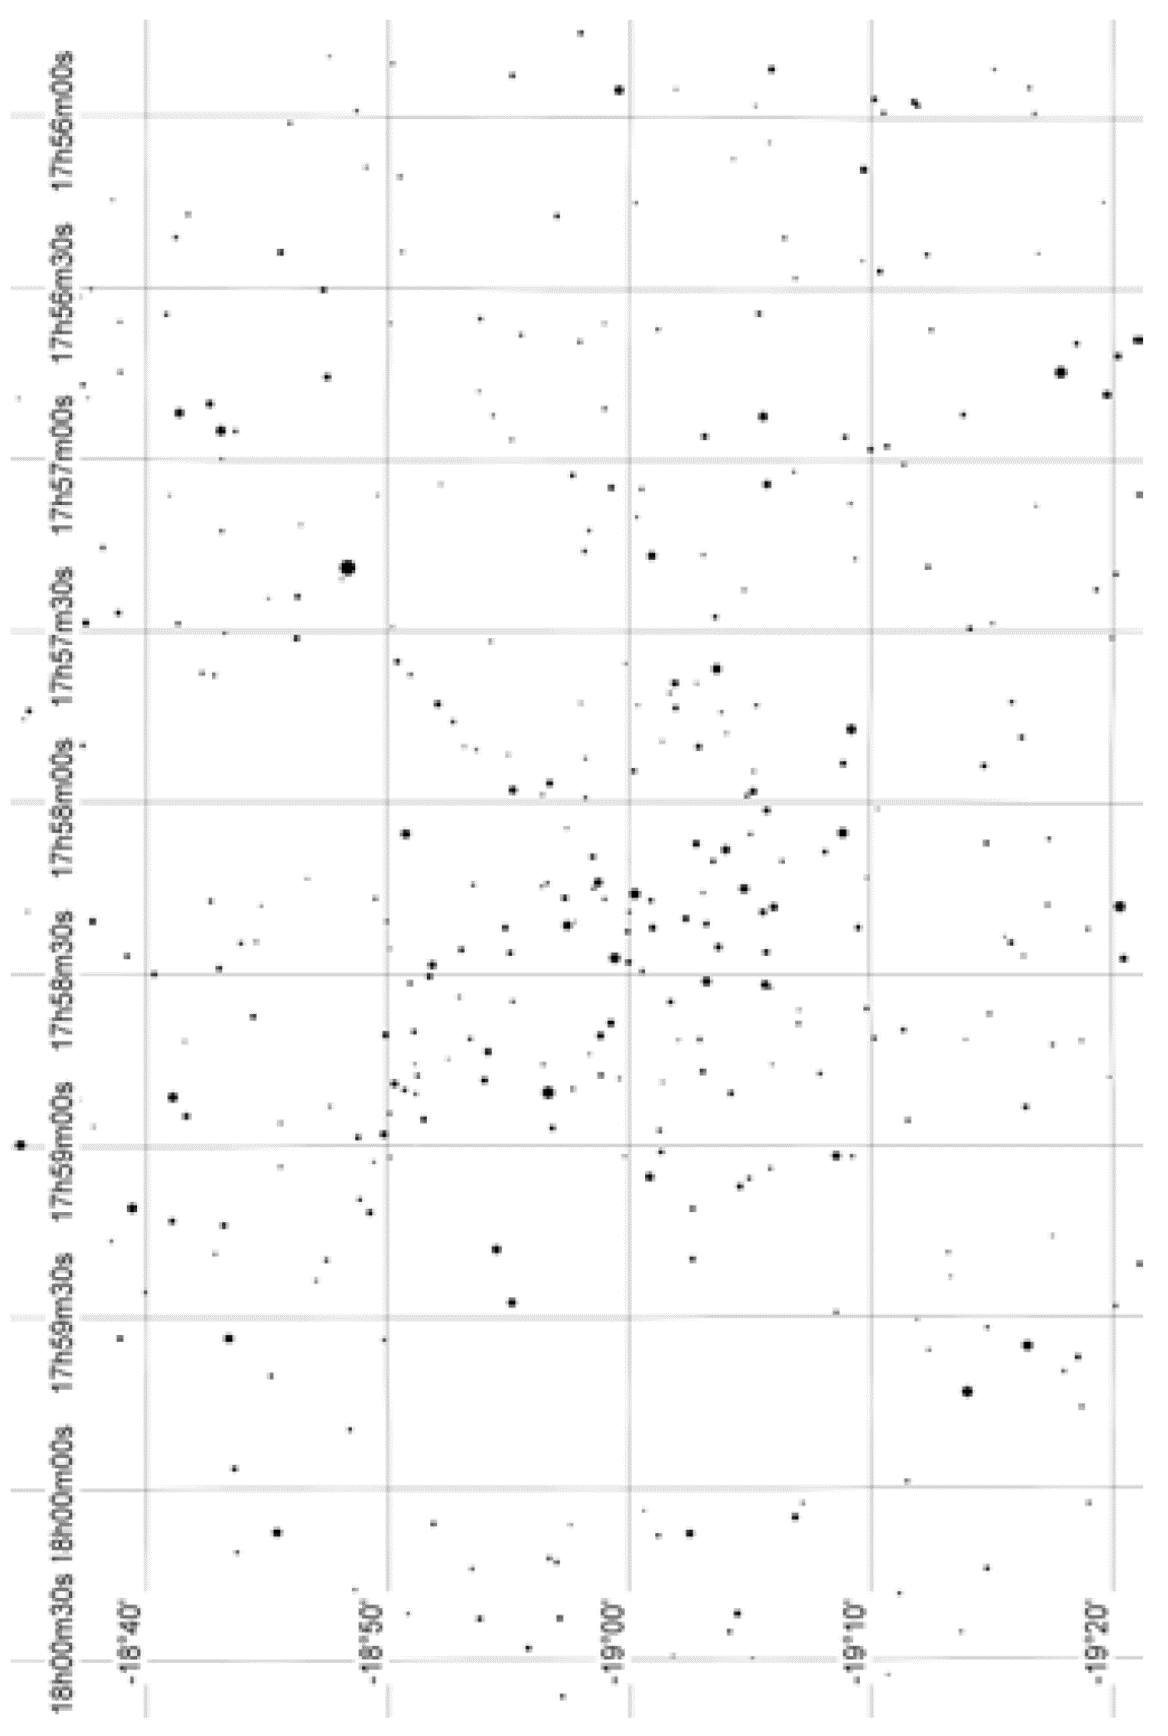
\includegraphics{fig/2.png}
	\end{figure}
	
	\newpage
	\section{小行星掩星}
	
	基于轨道根数的计算预测, 一颗小行星将掩食恒星HD 163390, 持续时间为21秒, 最大掩食 (中点时间) 发生在世界时23:03:32. 然而, 星历表并不完美, 预测的时间可能误差高达20秒, 持续时间可能误差高达10秒. 
	
	根据您的观测, 找出掩食的真实中点时间和持续时间. 使用星图1和以下坐标来识别这颗恒星:
	
	\hspace{1em}HD 163390\quad RA: $17^\text{h}$ $58^\text{m}$ $05^\text{s}$\,\, DEC: $-18^\circ$ $50'$ $46.14''$
	
	星图和天空处于同一历元. 
	
	\points{15}
	
	\vspace{0em}
	\textbf{\Large 答题纸}
	
	\begin{tabular}{|c|c|c|c|}
		\hline
		掩食中点时间 & $\pm$误差 & 掩食持续时间 & $\pm$误差 \\
		\hline
		& & & \\
		\hline
	\end{tabular}
	
	\vspace{1em}
	
	\section{星链}
	
	在与问题1相同的星场中, 在世界时大约23:05, 一列``星链''卫星将出现在$17^\text{h}$ $59^\text{m}$的子午线附近. 它们的通过将持续大约三分钟. 
	
	您可以假设星场中心的高度为$20^\circ$, 并且卫星在地球表面上方400 km, 以相等的距离在圆形轨道上移动. 您还可以假设卫星将垂直移动 (与地平线垂直) . 
	
	\begin{enumerate}[label=(\alph*)]
		\item 测量模拟天空中观察者看到的卫星的角速度. 
		
		\item 测量连续两颗卫星经过之间的时间间隔, 并在星图 (星图1) 上标记它们的路径. 
		
		\item 利用问题中给出的信息, 计算观察者看到的卫星的理论角速度. 
		
		\item 估计两个连续卫星之间的距离, 单位为km. 
	\end{enumerate}
	
	常数:$G=6.674\times10^{-11}\text{ N m}^2\text{ kg}^{-2}$;$M_\mathrm{Earth}=5.972\times10^{24}\text{ kg}$;$R_\mathrm{Earth}=6378\text{ km}$. 
	
	\points{15}
	
	\newpage
	\section{行星的卫星}
	
	屏幕上将展示2023年8月15日世界时00:00观测到的太阳系某颗行星的图像. 识别出五颗卫星并在答题卡上标记它们的位置 (您可以使用附在下方的卫星位置图表以及显示它们亮度的表格) . 
	\points{10}
	
	\vspace{0em}
	{\centering
		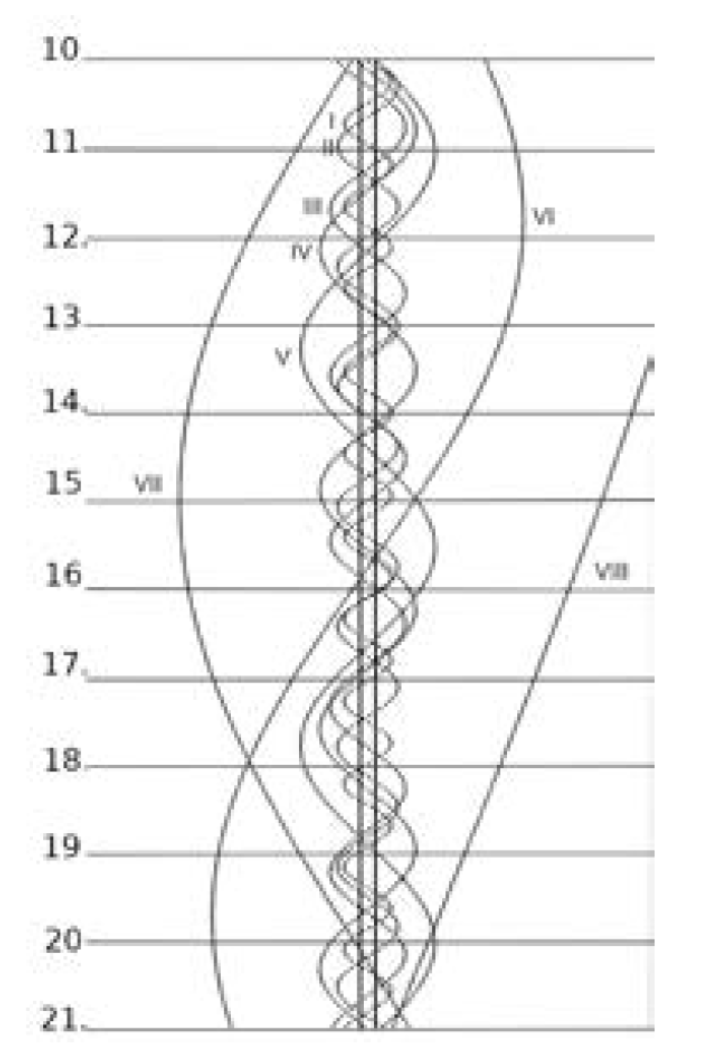
\includegraphics{fig/3.png}
		\begin{center}
			卫星相位图. 左侧的数字表示2023年8月的日期 (世界时午夜) . 
			\end{center}}
	
	\vspace{0em}
	\begin{table}[!h]
		\centering
		\begin{tabular}{llr}
			\toprule
			序号 & 名字 & 星等\\
			\midrule
			I&Mimas&13.0\\
			II & Enceladus & 11.8 \\
			III & Tethys & 10.4 \\
			IV & Dione & 10.6 \\
			V & Rhea & 9.9 \\
			VI & Titan & 8.5 \\
			VII & Hyperion & 14.4 \\
			VIII & Iapetus & 11.0 \\
			\bottomrule
		\end{tabular}
	\end{table}
	
	\newpage
	{
		\centering
		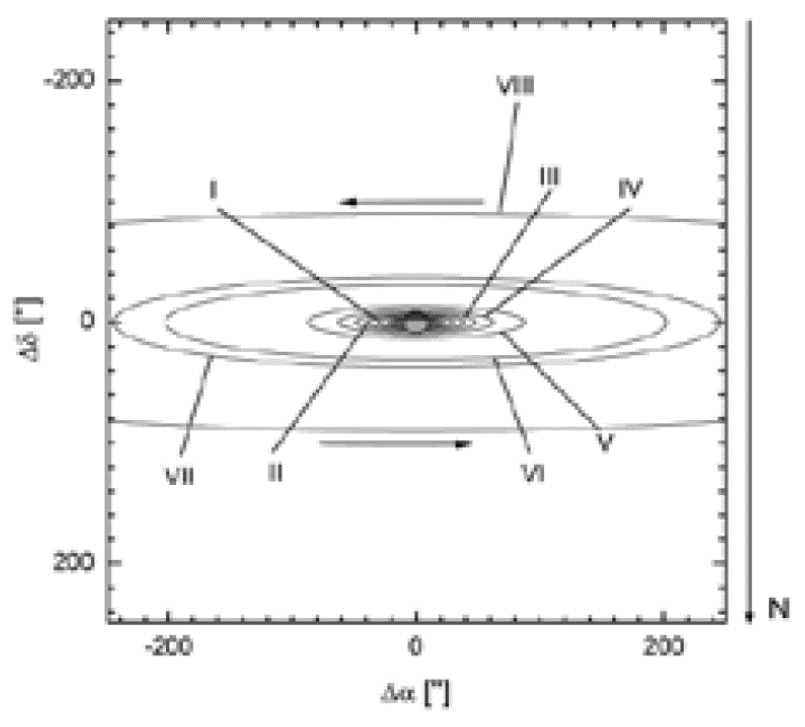
\includegraphics{fig/4.png}
		\begin{center}
			卫星相位图——卫星编号 (I、II、...) 如上. 
		\end{center}
	}
	
	\textbf{\Large 答题纸}
	
	在以下图像上用点标记任意5颗卫星的位置, 并用它们的编号 (I、II、...) 进行标注. 
	
	{\centering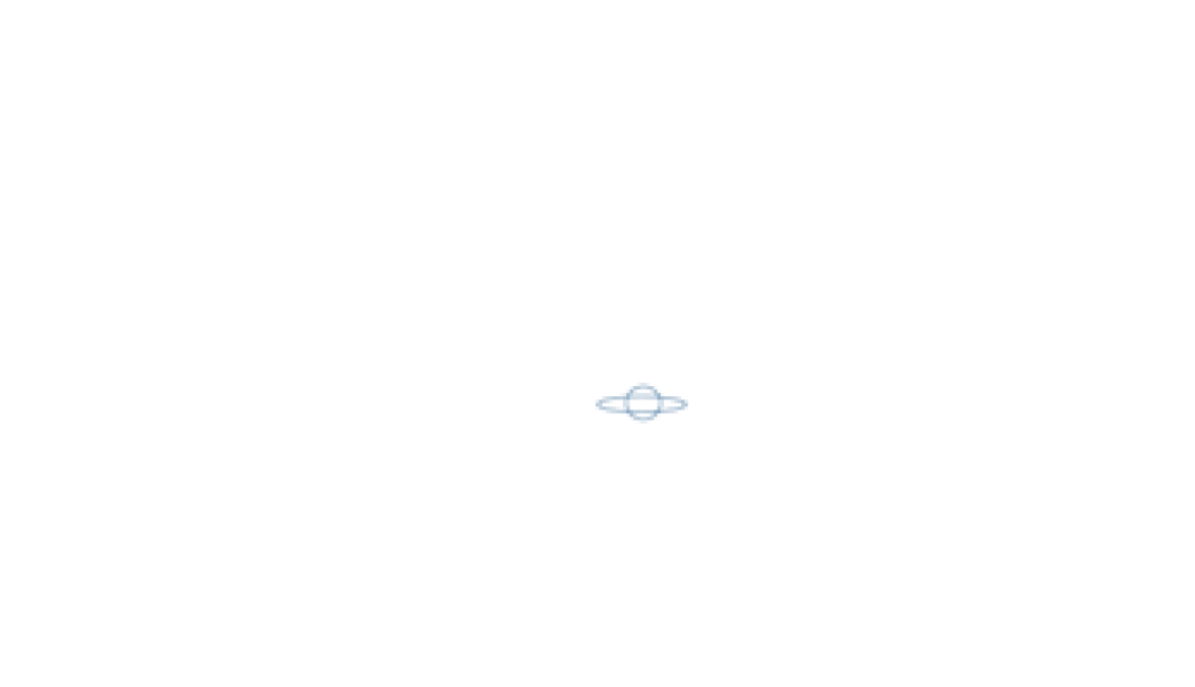
\includegraphics{fig/5.png}}
	
	\newpage
	\section{超新星}
	
	另一个屏幕上展示了一个星系的图像, 以及一个之前不可见的明亮 (星等 $< 11$) 天体. 估计这个恒星的赤经 (RA) 和赤纬 (DEC) 坐标, 并估计其星等. 您可以使用带有恒星坐标和星等列表的星图2. 
	\points{10}
	
	\vspace{0em}
	\begin{table}[!h]
		\centering
		\begin{tabular}{|l|rrr|rrr|r|}
			\hline
			恒星&\multicolumn{3}{|c|}{RA J2000}&\multicolumn{3}{|c|}{DEC J2000}&~~~~~~~~~~mag\\
			\hline
			&h&m&s&~~~~~~deg&m&s&\\
			\hline
			BD+69 541&9&55&2.7&68&56&22&10.3715\\
			Gaia DR2 1070097015969362560 & 9&53 & 27.9 & 68 & 58&43 & 11.2281 \\
			Gaia DR2 1070144329329069568 &9& 53 & 17.7 & 69 &2& 48 &10.0785  \\
			Gaia DR2 1070453463896461952 & 9 & 57 & 0.8 &  68 & 54 &6& 8.9148 \\
			Gaia DR2 1070455010084791680 &9& 55 & 25.9 & 68 & 51&21 & 11.4722 \\
			Gaia DR2 1070459408131196776 & 9 & 58 & 1.6 & 68 & 57 & 24 & 10.2003 \\
			Gaia DR2 1070467070352960512 & 9 & 55 & 4.4 & 68& 54 & 5 & 9.1615 \\
			Gaia DR2 1070467379590606976 & 9 & 55 & 1 & 68&56&22&10.4605 \\
			Gaia DR2 1070468169864590208 & 9 & 54 & 45.3 & 68 &56& 59 & 12.2097 \\
			Gaia DR2 1070469475534553728 & 9 & 55 & 41.4 & 69 & 0 & 30 & 11.7856 \\
			Gaia DR2 1070470265808536448 & 9 & 55 & 45 &69& 1 & 46 & 11.2905 \\
			Gaia DR2 1070470609404512512 & 9 & 55 & 33.2 & 69 & 3 & 55 & 13.3020 \\
			Gaia DR2 1070472293033168640 & 9 & 54 & 53.2 & 69 & 3 & 48 & 14.2845 \\
			Gaia DR2 1070473186386370176 & 9 & 54 & 42.3 & 69 & 5 & 52 & 11.6033 \\
			Gaia DR2 1070476794158817152 &9&57&38.8&69&10& 44  & 12.6348 \\
			Gaia DR2 1070476858581360384 &9& 56 & 47.1 & 69 & 7 & 27& 12.7250 \\
			Gaia DR2 1070476897238038272 & 9 & 56 & 34.4 & 69 & 7 & 51 & 13.6578 \\
			Gaia DR2 1070477240835421440 &9&56&44.8&69&9& 1 & 13.7626 \\
			Gaia DR2 1070477305257957888 & 9 & 56 & 45.1 & 69 & 10& 1 & 11.4495 \\
			Gaia DR2 1070522934990509312 & 9 &55&15.4&69&15&19& 12.0436 \\
			Gaia DR2 1070523111086221568 & 9 & 54&28.6 & 69 & 13 & 22 & 11.0704 \\
			HD85458 & 9& 55&4 & 68 & 54 &6& 9.1615 \\
			\hline
		\end{tabular}
	\end{table}
	
	\vspace{3em}
	\textbf{\Large 答题纸}
	
	\begin{tabular}{|c|c|c|}
		\hline
		赤经(RA) & 赤纬(DEC) & 估计星等 \\
		\hline
		&&\\
		\hline
	\end{tabular}
	
	\newpage
	{
		\Large\bfseries\noindent 观测:\hspace{0.5em}星图2
	}
	
	\begin{figure}[!h]
		\centering
		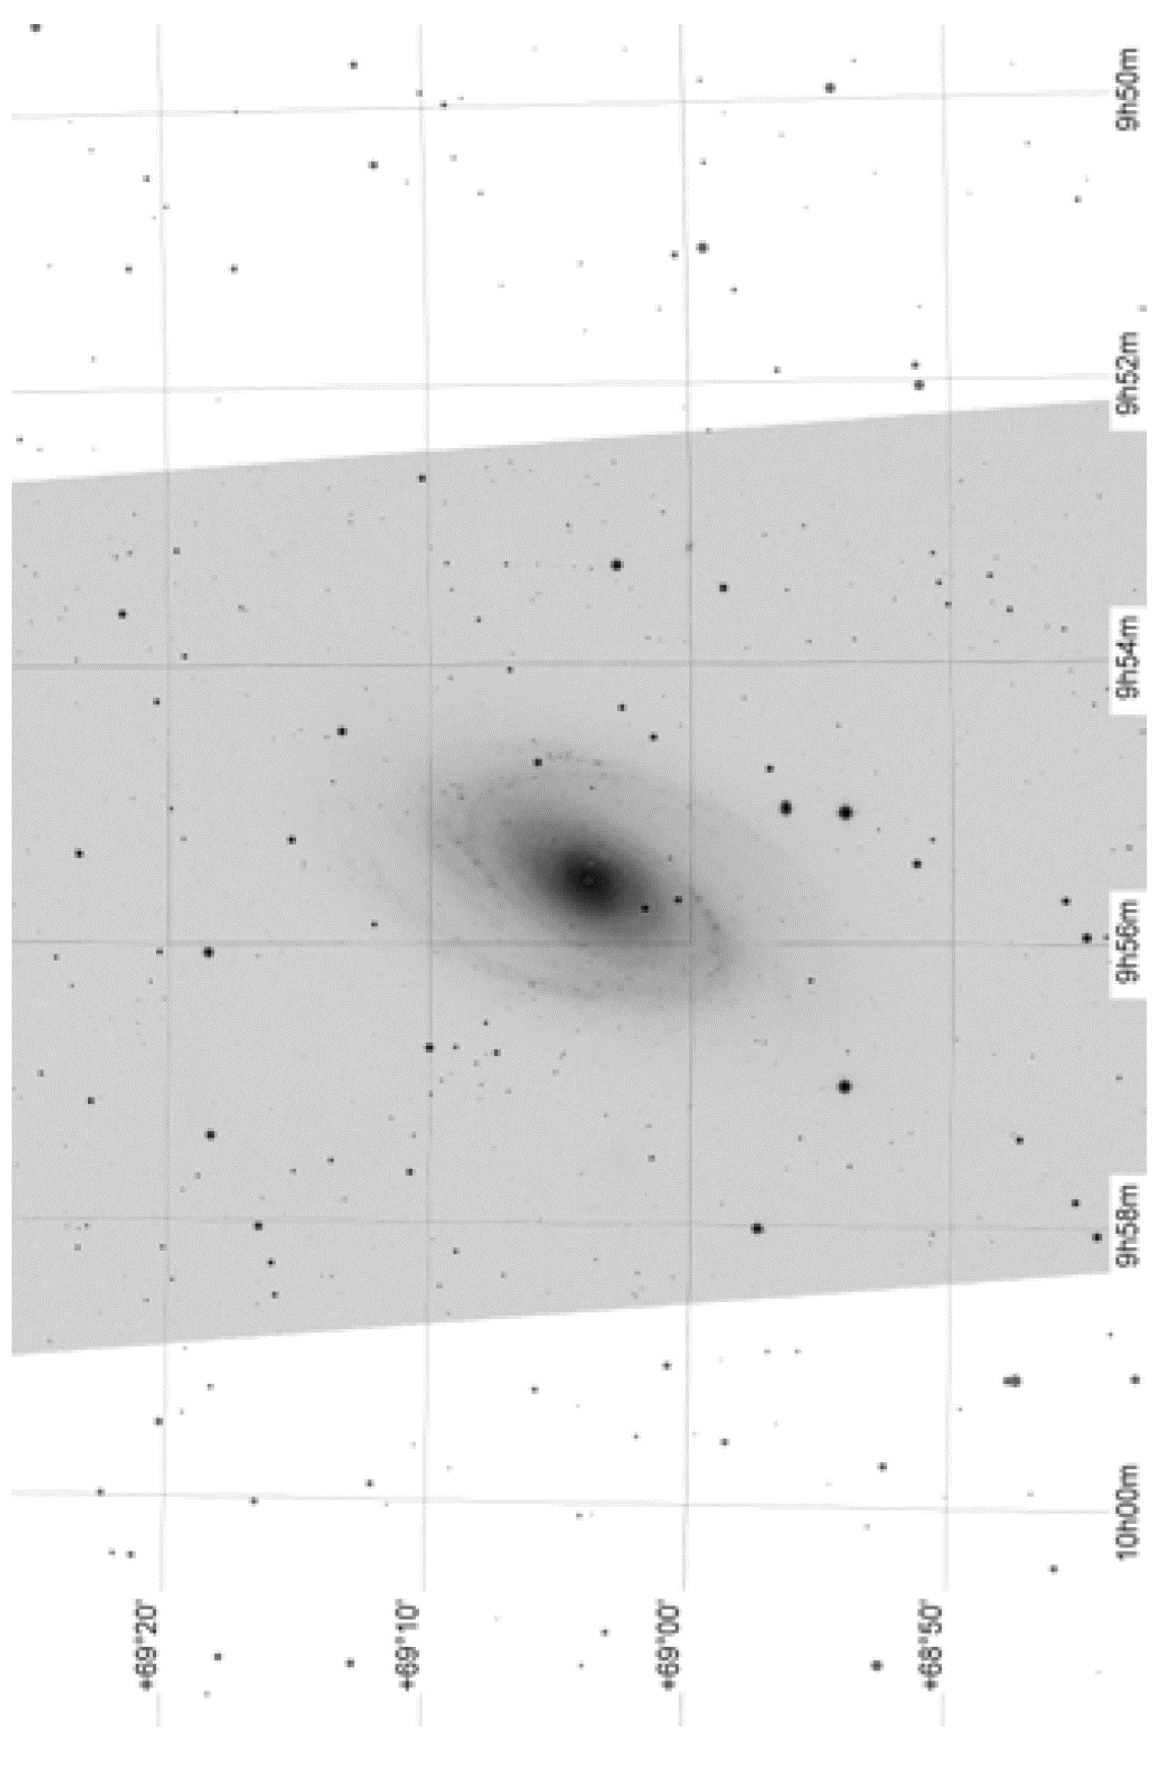
\includegraphics{fig/6.png}
	\end{figure}
	
\end{document}